\documentclass[compress]{beamer}
%\documentclass[ignorenonframetext,handout]{beamer}
%\setbeamercovered{transparent}
%\usepackage[ISO 8859-1]{inputenc}
\usepackage{default}
\usepackage{siunitx}
% para usar figuras devemos acrescentar
\usepackage{graphicx}
%\usepackage{graphics}
%\DeclareGraphicsExtensions{.pdf,.png,.jpg}
%\DeclareGraphicsExtensions{.jpg, .eps}
%\DeclareGraphicsRule{.jpg}{eps}{.jpg}{`jpeg2ps -h -r 600 #1}
\usepackage{tikz}
\usepackage{bm}
%\usetikzlibrary{arrows,backgrounds,coordinatesystems,3d,shapes,plotmarks,automata,calendar,er,
%folding,matrix,mindmap,patterns,petri,plothandlers,topaths,trees} 
\usetikzlibrary{positioning}
%\usepgflibrary{decorations.pathreplacing}
\usetikzlibrary{decorations.pathreplacing}
\usetikzlibrary{decorations.pathmorphing}
\usetikzlibrary[patterns]
%\tikzstyle{every text node part}
%\usetikzlibrary{arrows,backgrounds,positioning,fit} 
\usetikzlibrary{calc}
% para gerar graficos no latex
\usepackage{pgfplots}
\pgfplotsset{compat=newest}

\usepackage{amsfonts}
\usepackage{amssymb}
\usepackage{amsmath}
\usepackage{MnSymbol}

\usepackage[brazil]{babel}
\usepackage[utf8]{inputenc}

% \usepackage{algpseudocode}
% \usepackage{algorithmicx}
\usepackage[Algoritmo]{algorithm}
\usepackage[noend]{algorithmic}

%\usepackage{biblatex}


\setbeamertemplate{bibliography entry title}{}
\setbeamertemplate{bibliography entry location}{}
\setbeamertemplate{bibliography entry note}{}

\newcounter{saveenumi}
\newcommand{\seti}{\setcounter{saveenumi}{\value{enumi}}}
\newcommand{\conti}{\setcounter{enumi}{\value{saveenumi}}}

%\usepackage{shadethm}

%\definecolor{shadethmcolor}{rgb}{.75,.75,.75}

%\newshadetheorem{theorem}{\scshape Teorema}[chapter]
\newtheorem{teorema}[theorem]{\scshape Teorema}
\newtheorem{proposicao}[theorem]{\scshape Proposição}
\newtheorem{corolario}[theorem]{\scshape Corolário}
\newtheorem{lema}[theorem]{\scshape Lema}
\newtheorem{definicao}[theorem]{\scshape Definição}
\newtheorem{conjectura}[theorem]{\scshape Conjectura}
\newtheorem{escolio}[theorem]{\scshape Escólio}
\newtheorem{exemplo}[theorem]{\scshape Exemplo}
\newtheorem{exemplos}[theorem]{\scshape Exemplos}
\newtheorem{propriedade}[theorem]{\scshape Propriedade}

\renewcommand{\u}{{\bf u}}
\renewcommand{\v}{{\bf v}}
\renewcommand{\sin}{\operatorname{sen}}
\providecommand{\cas}{\operatorname{cas}}
\providecommand{\mdc}{\mathrm{mdc}}
\providecommand{\f}{{\bf f}}

\newcommand{\ie}{\textit{i.e.}}
\newcommand{\eg}{\textit{e.g.}}
%\newcommand{\qed}{\hfill $\square$}

\renewcommand\Re{\operatorname{Re}}
\renewcommand\Im{\operatorname{Im}}

\providecommand{\x}{{\bf x}}
\providecommand{\y}{{\bf y}}
\providecommand{\w}{{\bf w}}
\providecommand{\f}{{\bf f}}
\providecommand{\q}{{\bf q}}
\providecommand{\bfa}{{\bf a}}
\providecommand{\bfb}{{\bf b}}
\providecommand{\bfc}{{\bf c}}
\providecommand{\bfd}{{\bf d}}
\providecommand{\bfe}{{\bf e}}
\providecommand{\bfs}{{\bf s}}
\providecommand{\bfz}{{\bf z}}
\providecommand{\zero}{{\bf 0}}
\providecommand{\spn}{\mathrm{span}}
\providecommand{\posto}{\mathrm{posto}}
\providecommand{\nul}{\mathrm{nul}}
\providecommand{\proj}{\mathrm{proj}}
\providecommand{\tr}{\mathrm{tr}}
\providecommand{\sgn}{\mathrm{sgn}}

\providecommand{\cov}{\mathrm{cov}}

\providecommand{\dilation}{\mathcal{D}}
\providecommand{\erosion}{\mathcal{E}}
\providecommand{\open}{\mathcal{O}}
\providecommand{\close}{\mathcal{C}}

\newcommand*{\Bhat}{\skew{3}{\hat}{B}}

\mode<presentation>
{
  \setbeamertemplate{background canvas}[vertical shading][bottom=white!10,top=blue!10]
  \usetheme{Berkeley}
%  \usetheme{CambridgeUS}
%  \usetheme{Madrid}
%  \usetheme{Warsaw}
  \usefonttheme{serif} 
 % \usefonttheme[onlysmall]{structurebold}
  \setbeamertemplate{headline}{}
  
%   \setbeamercovered{invisible} % default
  \setbeamercovered{ transparent, again covered={\opaqueness{25}} } % =15%
%   \setbeamercovered{transparent=50}
%   \setbeamercovered{dynamic}

%   \setbeamercovered{again covered={\opaqueness<1->{25}}}
}

% copiado do site:
% http://latex-beamer-class.10966.n7.nabble.com/Covering-images-transparent-i-e-dimmed-figures-td1504
% . html
\usepackage{ifthen}

\makeatletter
\newcommand{\includecoveredgraphics}[2][]{
    \ifthenelse{\the\beamer@coveringdepth=1}{
        \tikz
            \node[inner sep=0pt,outer sep=0pt,opacity=0.15]
                {\includegraphics[#1]{#2}};
    }{
        \tikz
            \node[inner sep=0pt,outer sep=0pt]
                {\includegraphics[#1]{#2}};%
    }
} 
\makeatother % não sei se precisa...


% para a disciplina de Processamento de Imagens
\title{Tratamento e Mineração de Dados}
\subtitle{Naive Bayes e Florestas Randômicas}
\author{Marcos Pereira}

\DeclareMathOperator{\e}{e}

\usepackage{minted}


\begin{document}


\frame{\titlepage}

%%% SUMÁRIO %%%
\frame{\tableofcontents}
\section{}
%\begin{frame}{Sumário}
%\begin{enumerate}
%\item Teoria
%\item Algoritmo
%\item Programa
%\item Resultados
%\item Animações
%\end{enumerate}
%\end{frame}
%\begin{frame}{\tableofcontents}
%\end{frame}

%%%%%%%%%%%%%%%%%%%%%%%%%%%%%%
\begin{frame}{Abordagem Teórica}
    \section{Abordagem Teórica}
    \subsection*{Considerações}
    \begin{align*}
        \mathbf{R}=\begin{array}{cc}
             \text{classe} \\
             \left[\begin{array}{ccc|c}
                  x_1& x_2&x_3& y_1\\
                  x'_1& x'_2&x'_3&y_2\\
                  x_1& x'_2&x_3&y_3\\
             \end{array}\right]\Bigg\}_{\text{instâncias}}
        \end{array}\begin{array}{c}\\=\begin{bmatrix}\mathbf{x}_1\\\mathbf{x}_2\\\mathbf{x}_3\end{bmatrix}\end{array}
    \end{align*}
    
    Desse modo os vetores instâncias são os vetores $\mathbf{x}_i$, é importante notar que as relações equivalem aos nossos data sets.
\end{frame}
\begin{frame}{ML}
    \subsection{Aprendizado Supervisionado (ML)}
    \begin{itemize}
        \item Criar modelos genéricos;
        \item Evitar a criação de modelos superajustados;
        \item Treinar o modelo e testá-lo. Como?
    \end{itemize}
\end{frame}

%figuras

\begin{frame}{}
    \begin{figure}
        \centering
        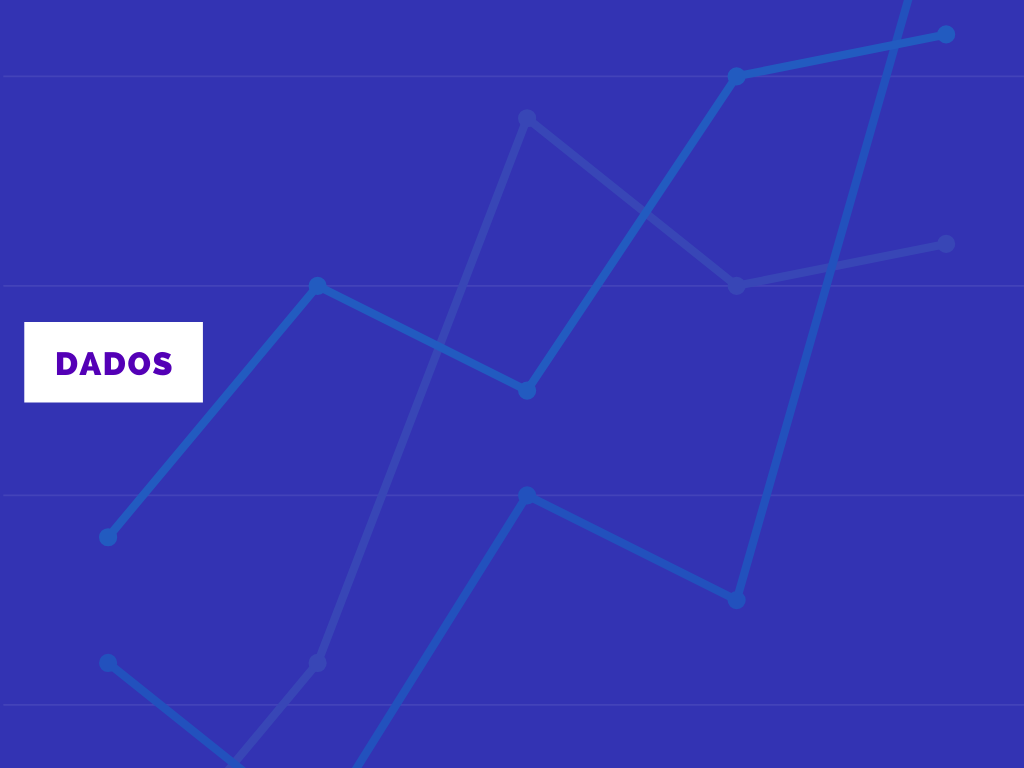
\includegraphics[scale=.39]{img/1.png}
    \end{figure}
\end{frame}
\begin{frame}{}
    \begin{figure}
        \centering
        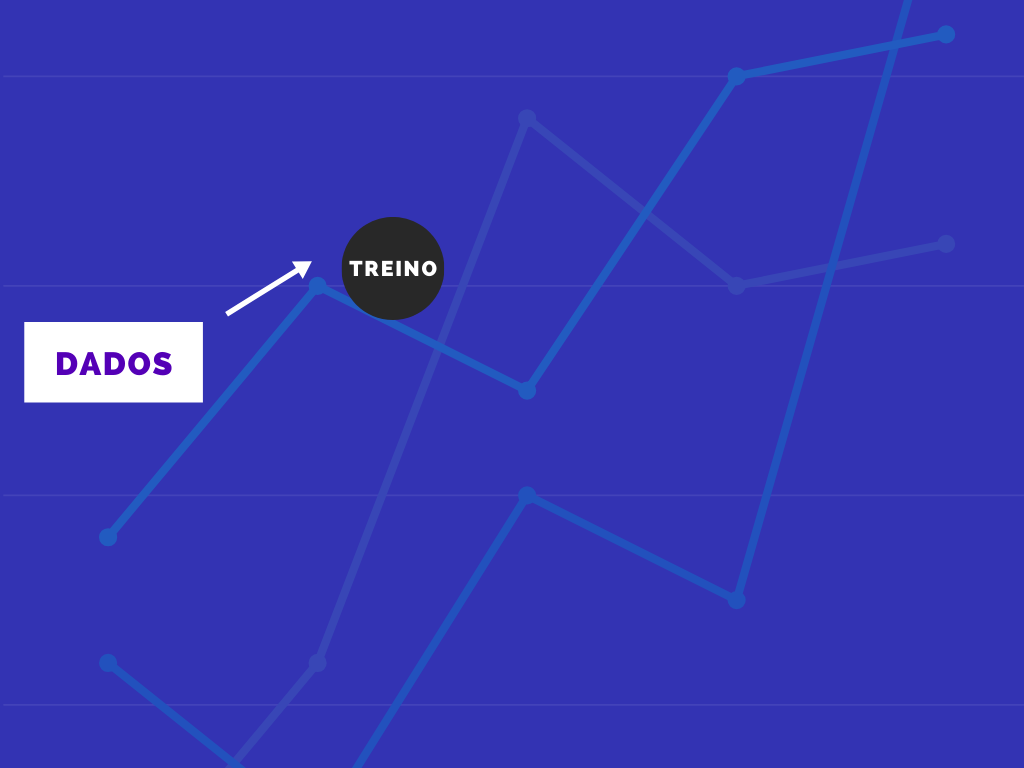
\includegraphics[scale=.39]{img/2.png}
    \end{figure}
\end{frame}

\begin{frame}{}
    \begin{figure}
        \centering
        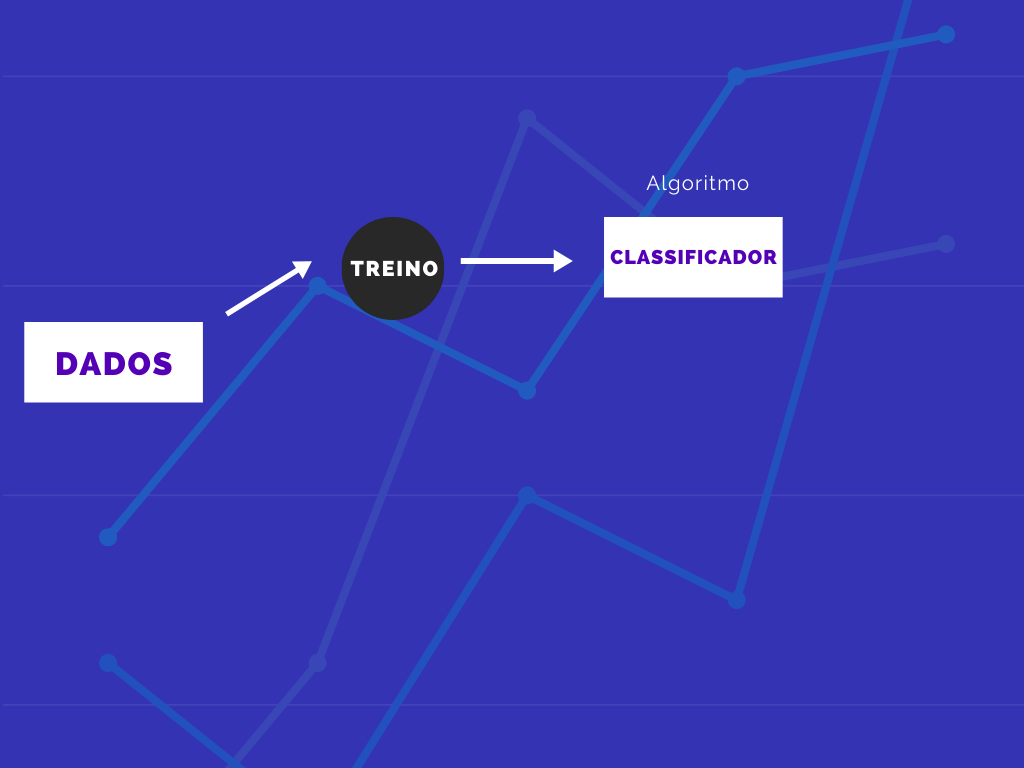
\includegraphics[scale=.39]{img/3.png}
    \end{figure}
\end{frame}
\begin{frame}{}
    \begin{figure}
        \centering
        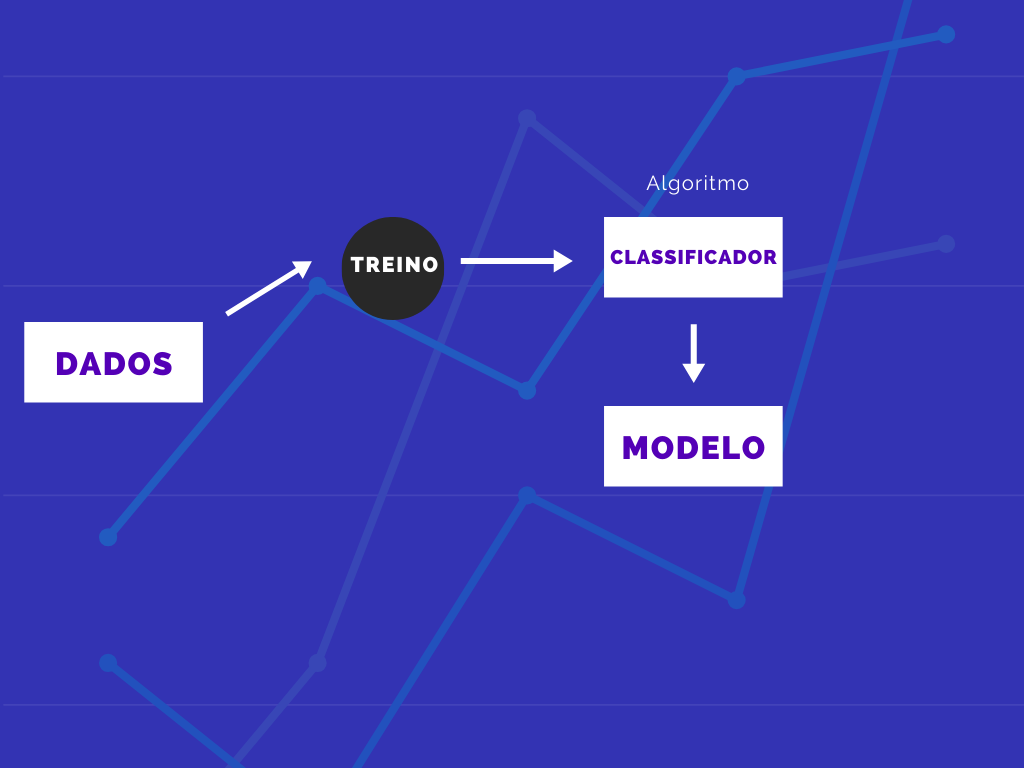
\includegraphics[scale=.39]{img/4.png}
    \end{figure}
\end{frame}
\begin{frame}{}
    \begin{figure}
        \centering
        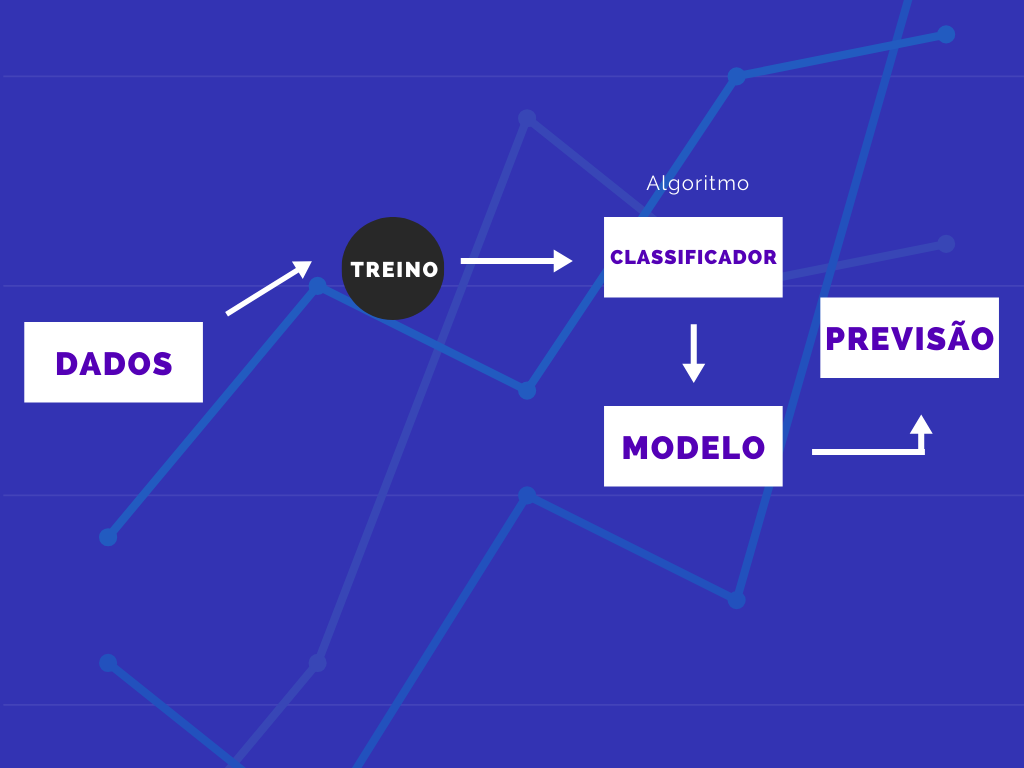
\includegraphics[scale=.39]{img/5.png}
    \end{figure}
\end{frame}
\begin{frame}{}
    \begin{figure}
        \centering
        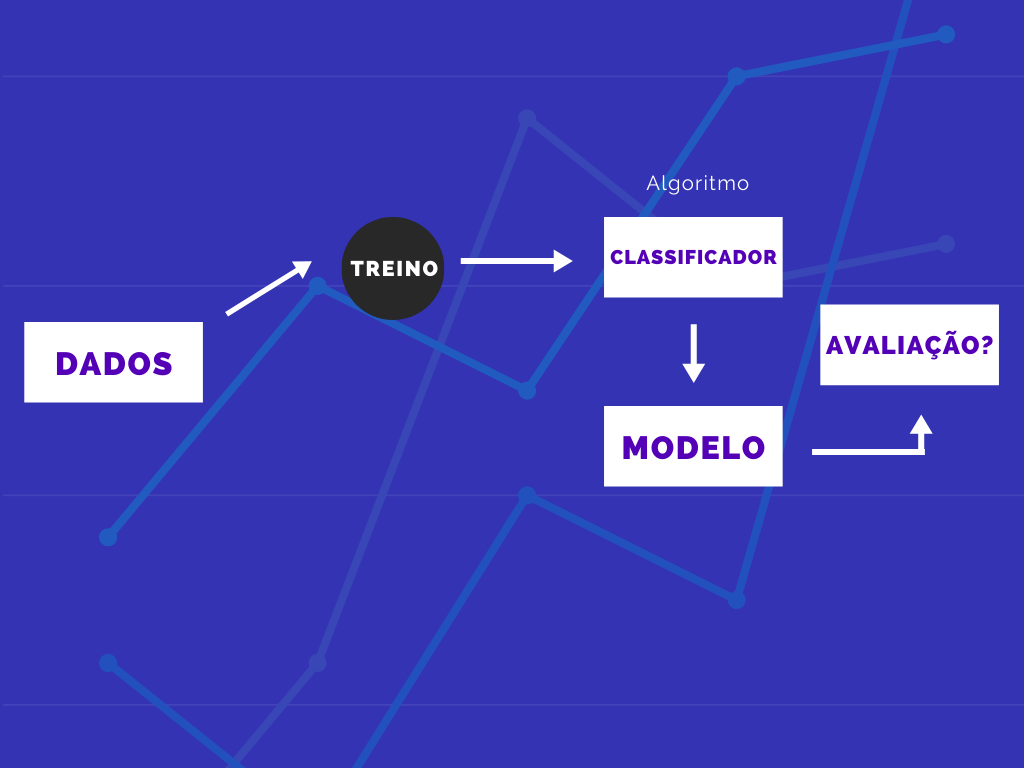
\includegraphics[scale=.39]{img/6.png}
    \end{figure}
\end{frame}
\begin{frame}{}
    \begin{figure}
        \centering
        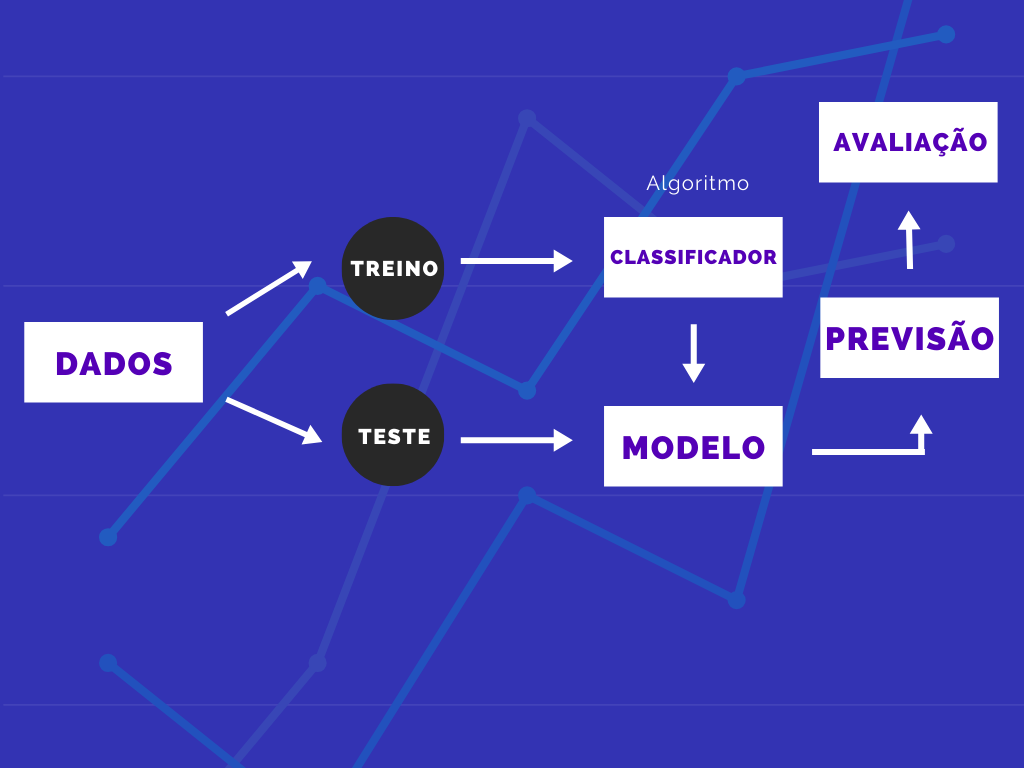
\includegraphics[scale=.39]{img/7.png}
    \end{figure}
\end{frame}
\begin{frame}{}
    \begin{figure}
        \centering
        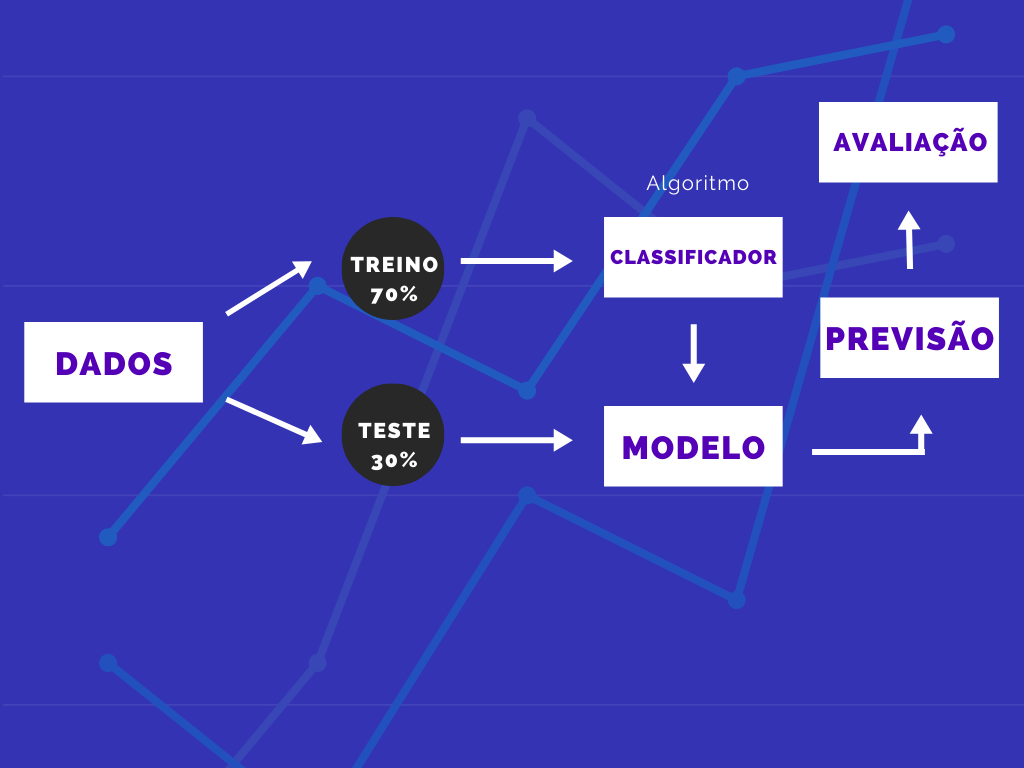
\includegraphics[scale=.39]{img/8.png}
    \end{figure}
\end{frame}
\begin{frame}{}
    \begin{figure}
        \centering
        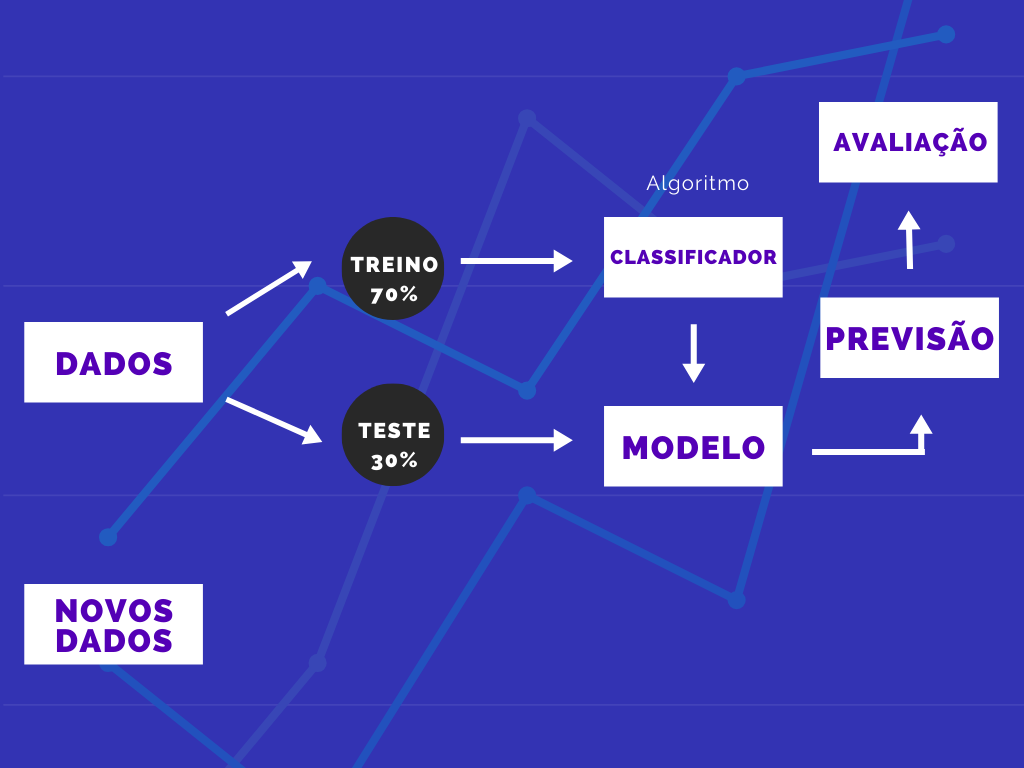
\includegraphics[scale=.39]{img/9.png}
    \end{figure}
\end{frame}
\begin{frame}{}
    \begin{figure}
        \centering
        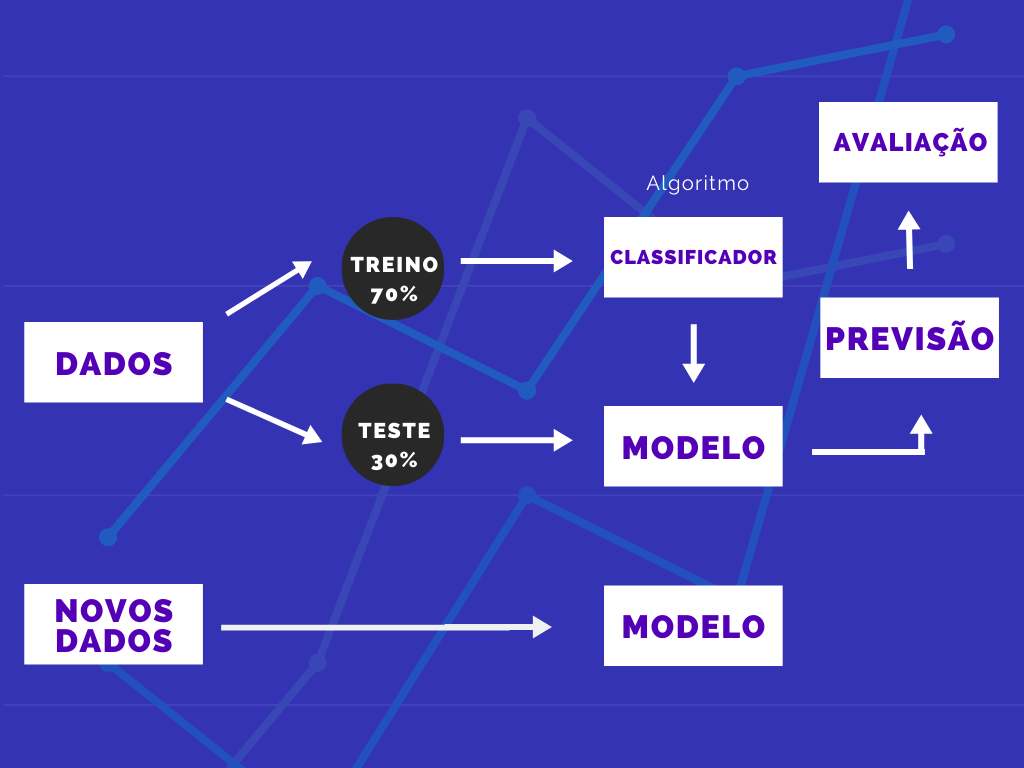
\includegraphics[scale=.39]{img/10.png}
    \end{figure}
\end{frame}

\begin{frame}{Abordagem Teórica}
\subsection{Naive Bayes}
\begin{itemize}
    \item Conjunto de Algoritmos de aprendizado supervisionado;
    \item Utiliza inferência Bayesiana
    \begin{itemize}
        \item Avaliação de hipóteses pela máxima verossimilhança
    \end{itemize}
    \item Teorema de Bayes\footnote{O símbolo $\prod$ representa um produtório.}: \begin{align}
    P\left(y|x_{1},\cdots,x_{2}\right)&=\prod_{i=1}^{n}\frac{P(y)P(x_i|y)}{P(x_i)}\\
    &\equiv \frac{P(y)\left(P(x_1|y)P(x_2|y)\cdots P(x_n|y)\right)}{P(x_1)P(x_2)\cdots P(x_n)}\nonumber
    \end{align}
    \item $P(\mathbf{x})\in\mathbb{R}$ (é constante), então utilizamos a seguinte regra de classificação:
    \begin{align}
        P(y|\mathbf{x})\propto \prod_{i=1}^{n}P(y)P(x_i|y)
    \end{align}
\end{itemize}
\end{frame}

\begin{frame}{}
    \begin{itemize}
        \item Máxima Probabilidade A Posteriori para realizar predição de dados:
        \begin{align}
            Y=\arg \max_{y} \prod_{i=1}^{n}P(y)P(x_i|y)
        \end{align}
        \item Naive Bayes Gaussiano. Verossimilhança\cite{scikit-learn}:
        $$P\left(x_i|y\right)=\frac{1}{\sqrt{2\pi}\sigma_{y}}\exp\left[-\left(\frac{x_i-\mu_y}{\sqrt{2}\sigma_y}\right)^2\right]$$
        \item Predição de dados:
        $$\displaystyle Y=\arg \max_{y}P(y)\exp\left[-\frac{1}{2\sigma_y^2}\sum_{i=1}\left(x_i-\mu_y\right)^2\right]$$
    \end{itemize}
\end{frame}


\begin{frame}{Floresta Randômica}
\begin{itemize}
    \item Ensemble Learning: Combinar predições de vários métodos de classificação a fim de otimizar a predição dos dados;
    \item Realizaremos a combinação de vários classificadores independentes, o resultado é a média das predições obtidas;
    \item Floresta Randômica: Baseado em árvores de decisão, consiste em criarmos $n$ árvores de decisão, treiná-las e obter a resposta de cada uma delas;
    \item Várias fontes de aleatoriedade reduzem a variância do "forest estimator", árvores de decisão sozinhas apresentam uma alta variância e consquentemente produzem modelos superajustados;
\end{itemize}
    
\end{frame}


\begin{frame}{}
    \begin{itemize}
        \item Implementação do Método será realizado utilizando o Sklearn \cite{scikit-learn}
    \end{itemize}
\end{frame}

\section{Implementação do Código}

Importação das bibliotecas e métodos:

\begin{minted}{python}
import numpy as np
import pandas as pd

from datetime import datetime

import matplotlib.pyplot as plt

import seaborn as sns


\end{minted}

em seguida os algoritmos e métodos de Machine Learning do sklearn:


\begin{minted}{python}
#ML

from sklearn.preprocessing import LabelEncoder,
OneHotEncoder

from sklearn.compose import make_column_transformer



#Divisão dados de treino e teste
from sklearn.model_selection import train_test_split

#Florestas Aleatórias

from sklearn.ensemble import RandomForestClassifier


#Método de Naive Bayes
from sklearn.naive_bayes import GaussianNB

#Taxa de acerto e de erro

from sklearn.metrics import accuracy_score

#Visualizaremos a matriz de confusão através da
#Yellow Brick
from yellowbrick.classifier import ConfusionMatrix
\end{minted}

Em seguidas começamos o tratamento dos dados, importando o dataset usando pandas

\begin{minted}{python}
    df=pd.read_csv('Data_Base.csv',encoding = 'ISO-8859-1')
    
    df.head()
\end{minted}
então verificamos que a tabela encontra-se sem informação com relação aos atributos ou até mesmo em relação à classe.

Levantar suposição com base nos dados contidos no Data Frame.

\begin{frame}{}
\begin{figure}[h!]
    \centering
    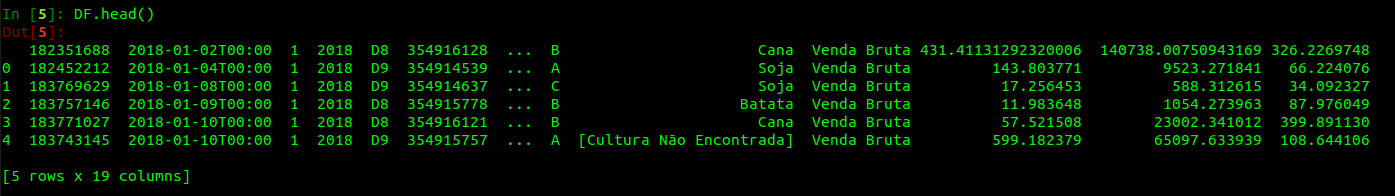
\includegraphics[scale=.2]{img/dfhead.png}
\end{figure}

Definir nome aos atributos para realizar a análise:
\end{frame}

\begin{minted}{python}
colunas = ['ID', 'Data/Hora Dia',  'Mês',
    'Ano', 'D#', 'Código', 'Código 2',
    'Código 3', 'Tipo de venda', 'UF',
    'Código 4', 'Família', 'Produto 1',
    'ABC',  'Produto 2', 'Venda Bruta col',
    'Venda Bruta 1', 'Venda Bruta 2',
    'Venda Bruta 3']
    
df = pd.read_csv('Data_Base.csv',names=colunas,
encoding = 'ISO-8859-1')    
    
\end{minted}

\begin{frame}{}
    \begin{itemize}
        \item Transformar segundo atributo no formato datetime;
        \item Remover atributos que são invariantes;
        \item Analisar uma visualização dos dados a partir da matriz de correlação;
        \item Analisar o plot dos pares;
    \end{itemize}
\end{frame}

\begin{minted}{python}
YmdHM = (lambda x: datetime.strptime(x,
        '%Y-%m-%dT%H:%M'))

#Year month day hour minute
#converter coluna em formato datetime

df['Data/Hora Dia'] =
    df['Data/Hora Dia'].apply(YmdHM)

#Verificar quais colunas possuem valores
#que não se repetem e remover

verificar = [len(df.iloc[:,i].value_counts().values)
        for i in range(len(df.columns.values))]

unit, index = -1, []
for i in verificar: 
  unit+=1 
  print('verificando {}'.format(colunas[unit]))
  if i==1:
    index.append(unit)
    df.drop(colunas[unit], axis=1,
    inplace=True)
    print('Coluna {} removida'
    .format(colunas[unit]))
    #colunas.remove(colunas[unit])

for i in index:
  colunas.remove(colunas[i])

#remover 'Mês'
colunas.remove('Mês')

df.drop('Mês', inplace=True, axis=1)
\end{minted}

\begin{frame}{Correlação}
    \begin{figure}[h!]
        \centering
        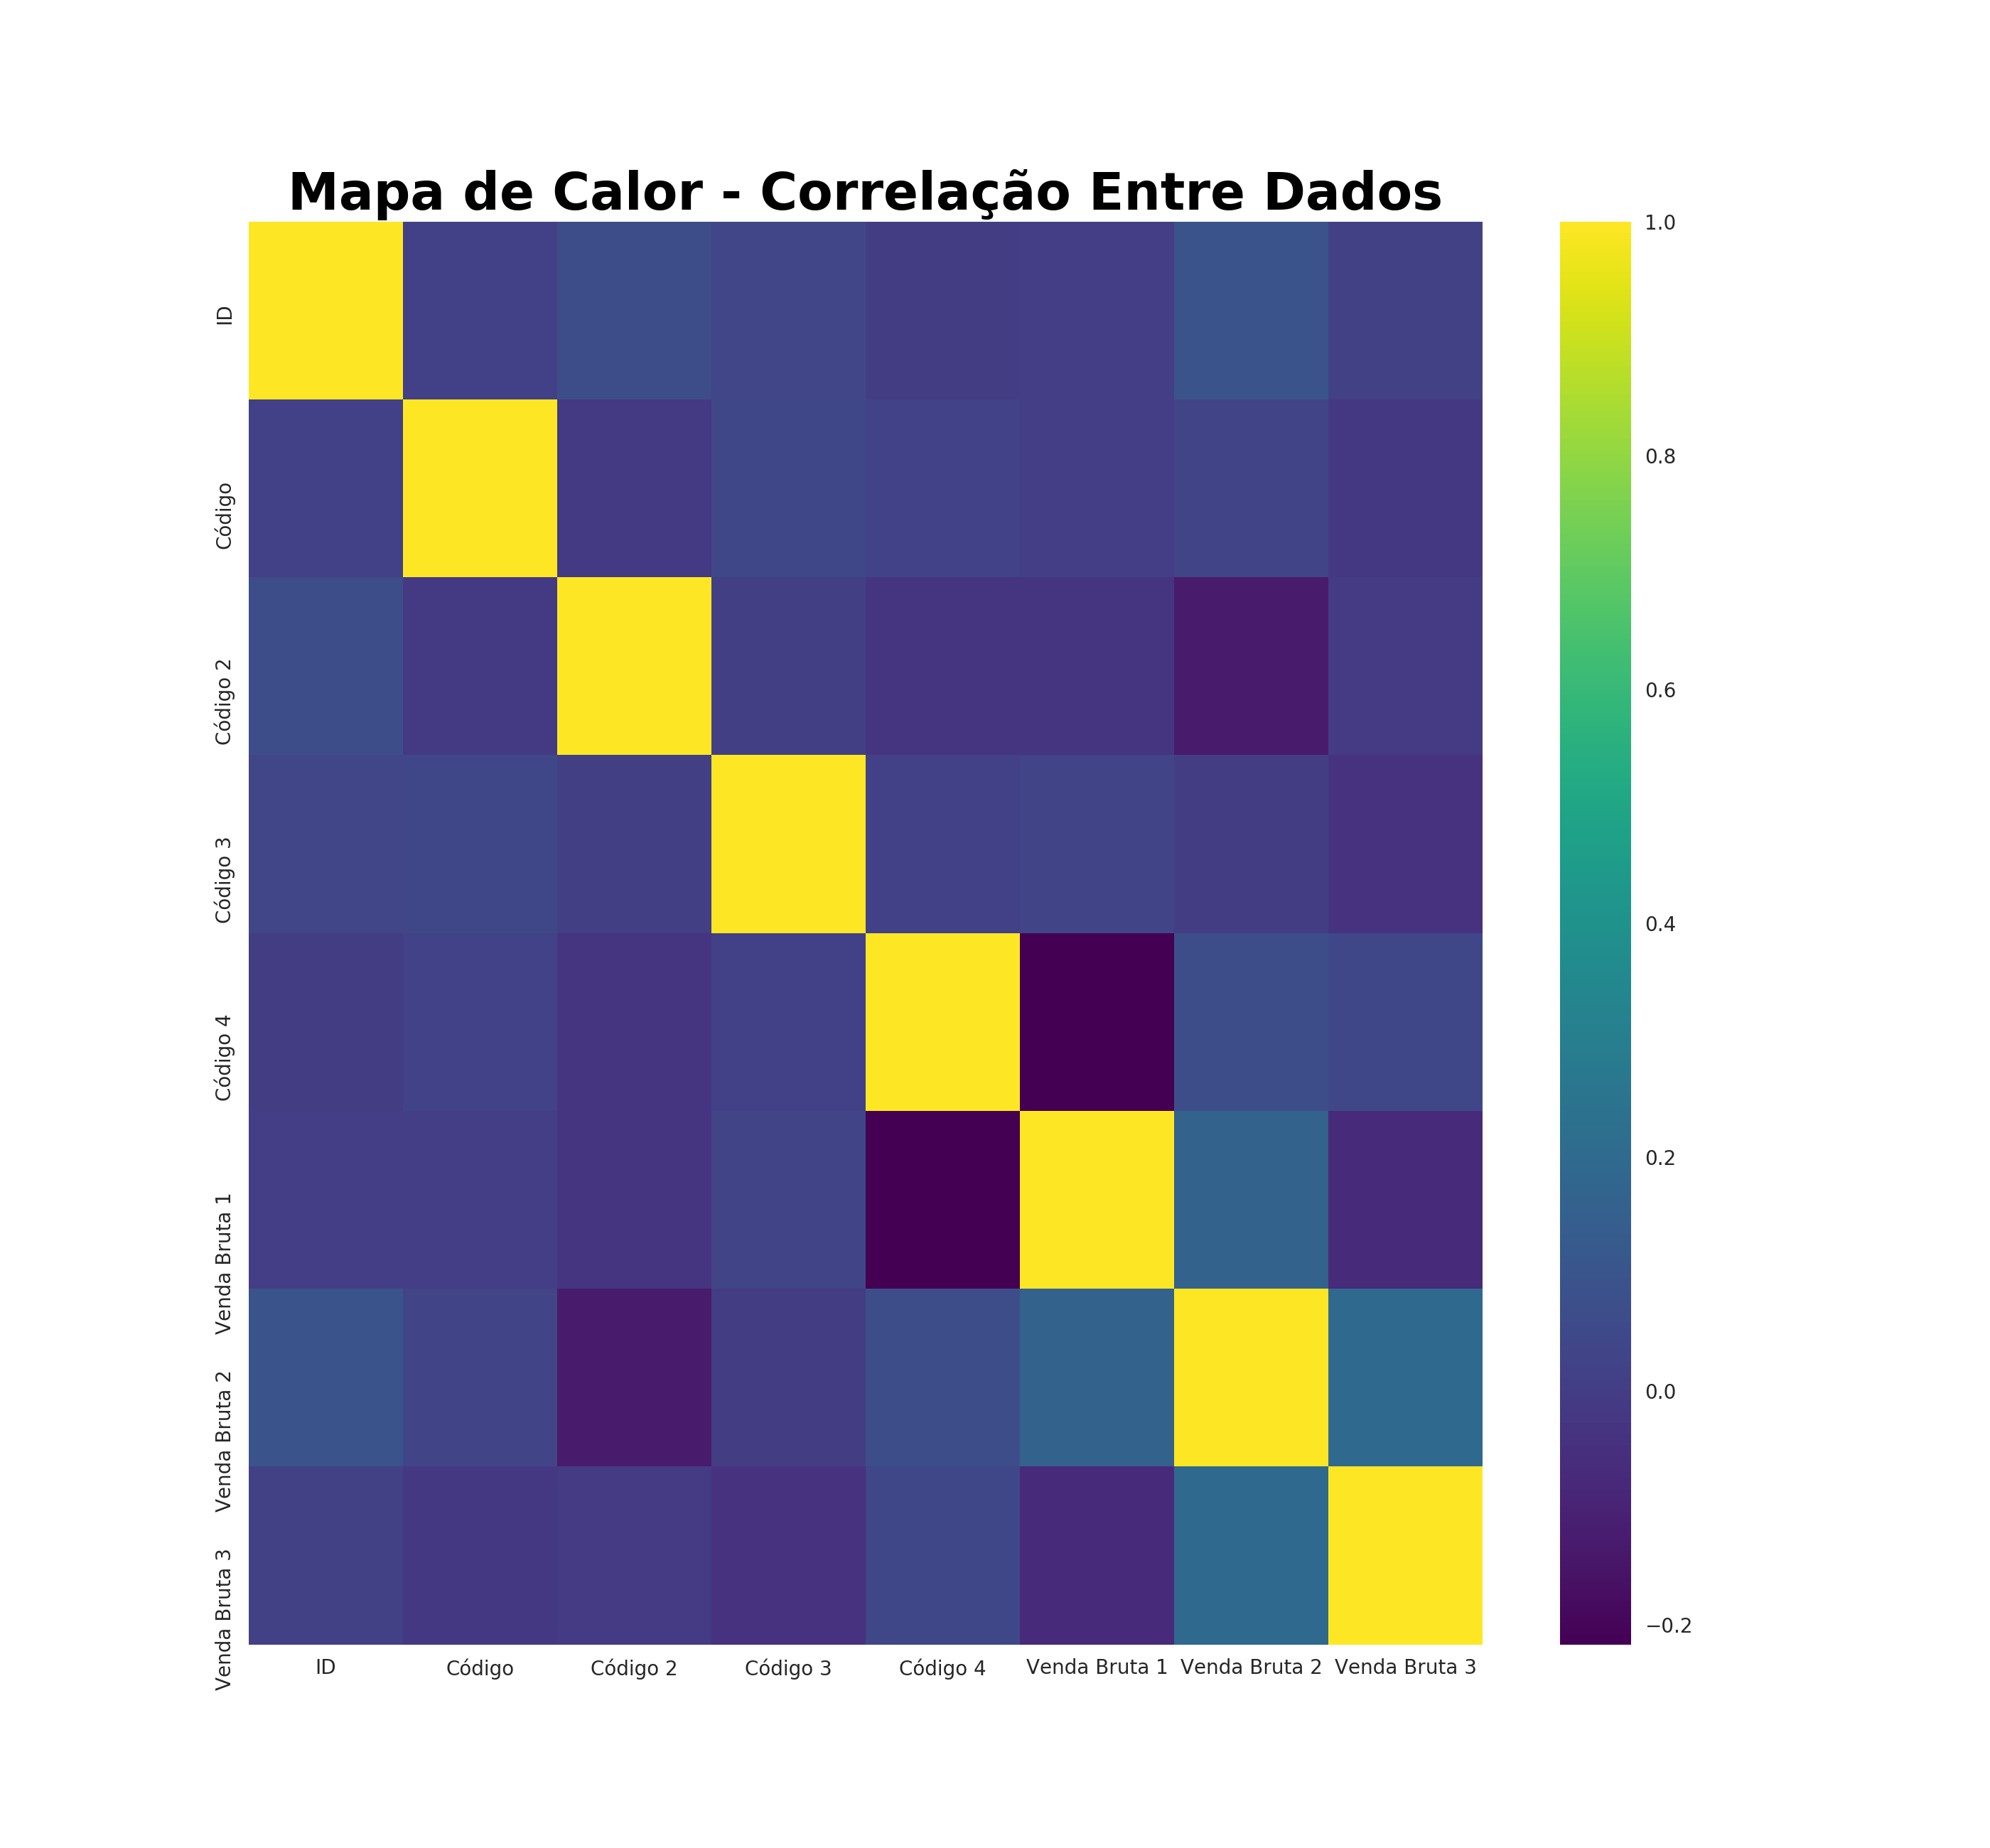
\includegraphics[scale=.25]{img/heatmap.png}
        \caption{Atributos não estão fortemente correlacionados;}
        \label{fig:corr}
    \end{figure}
\end{frame}
\begin{frame}{PairPlots}
    \begin{figure}[h!]
        \centering
        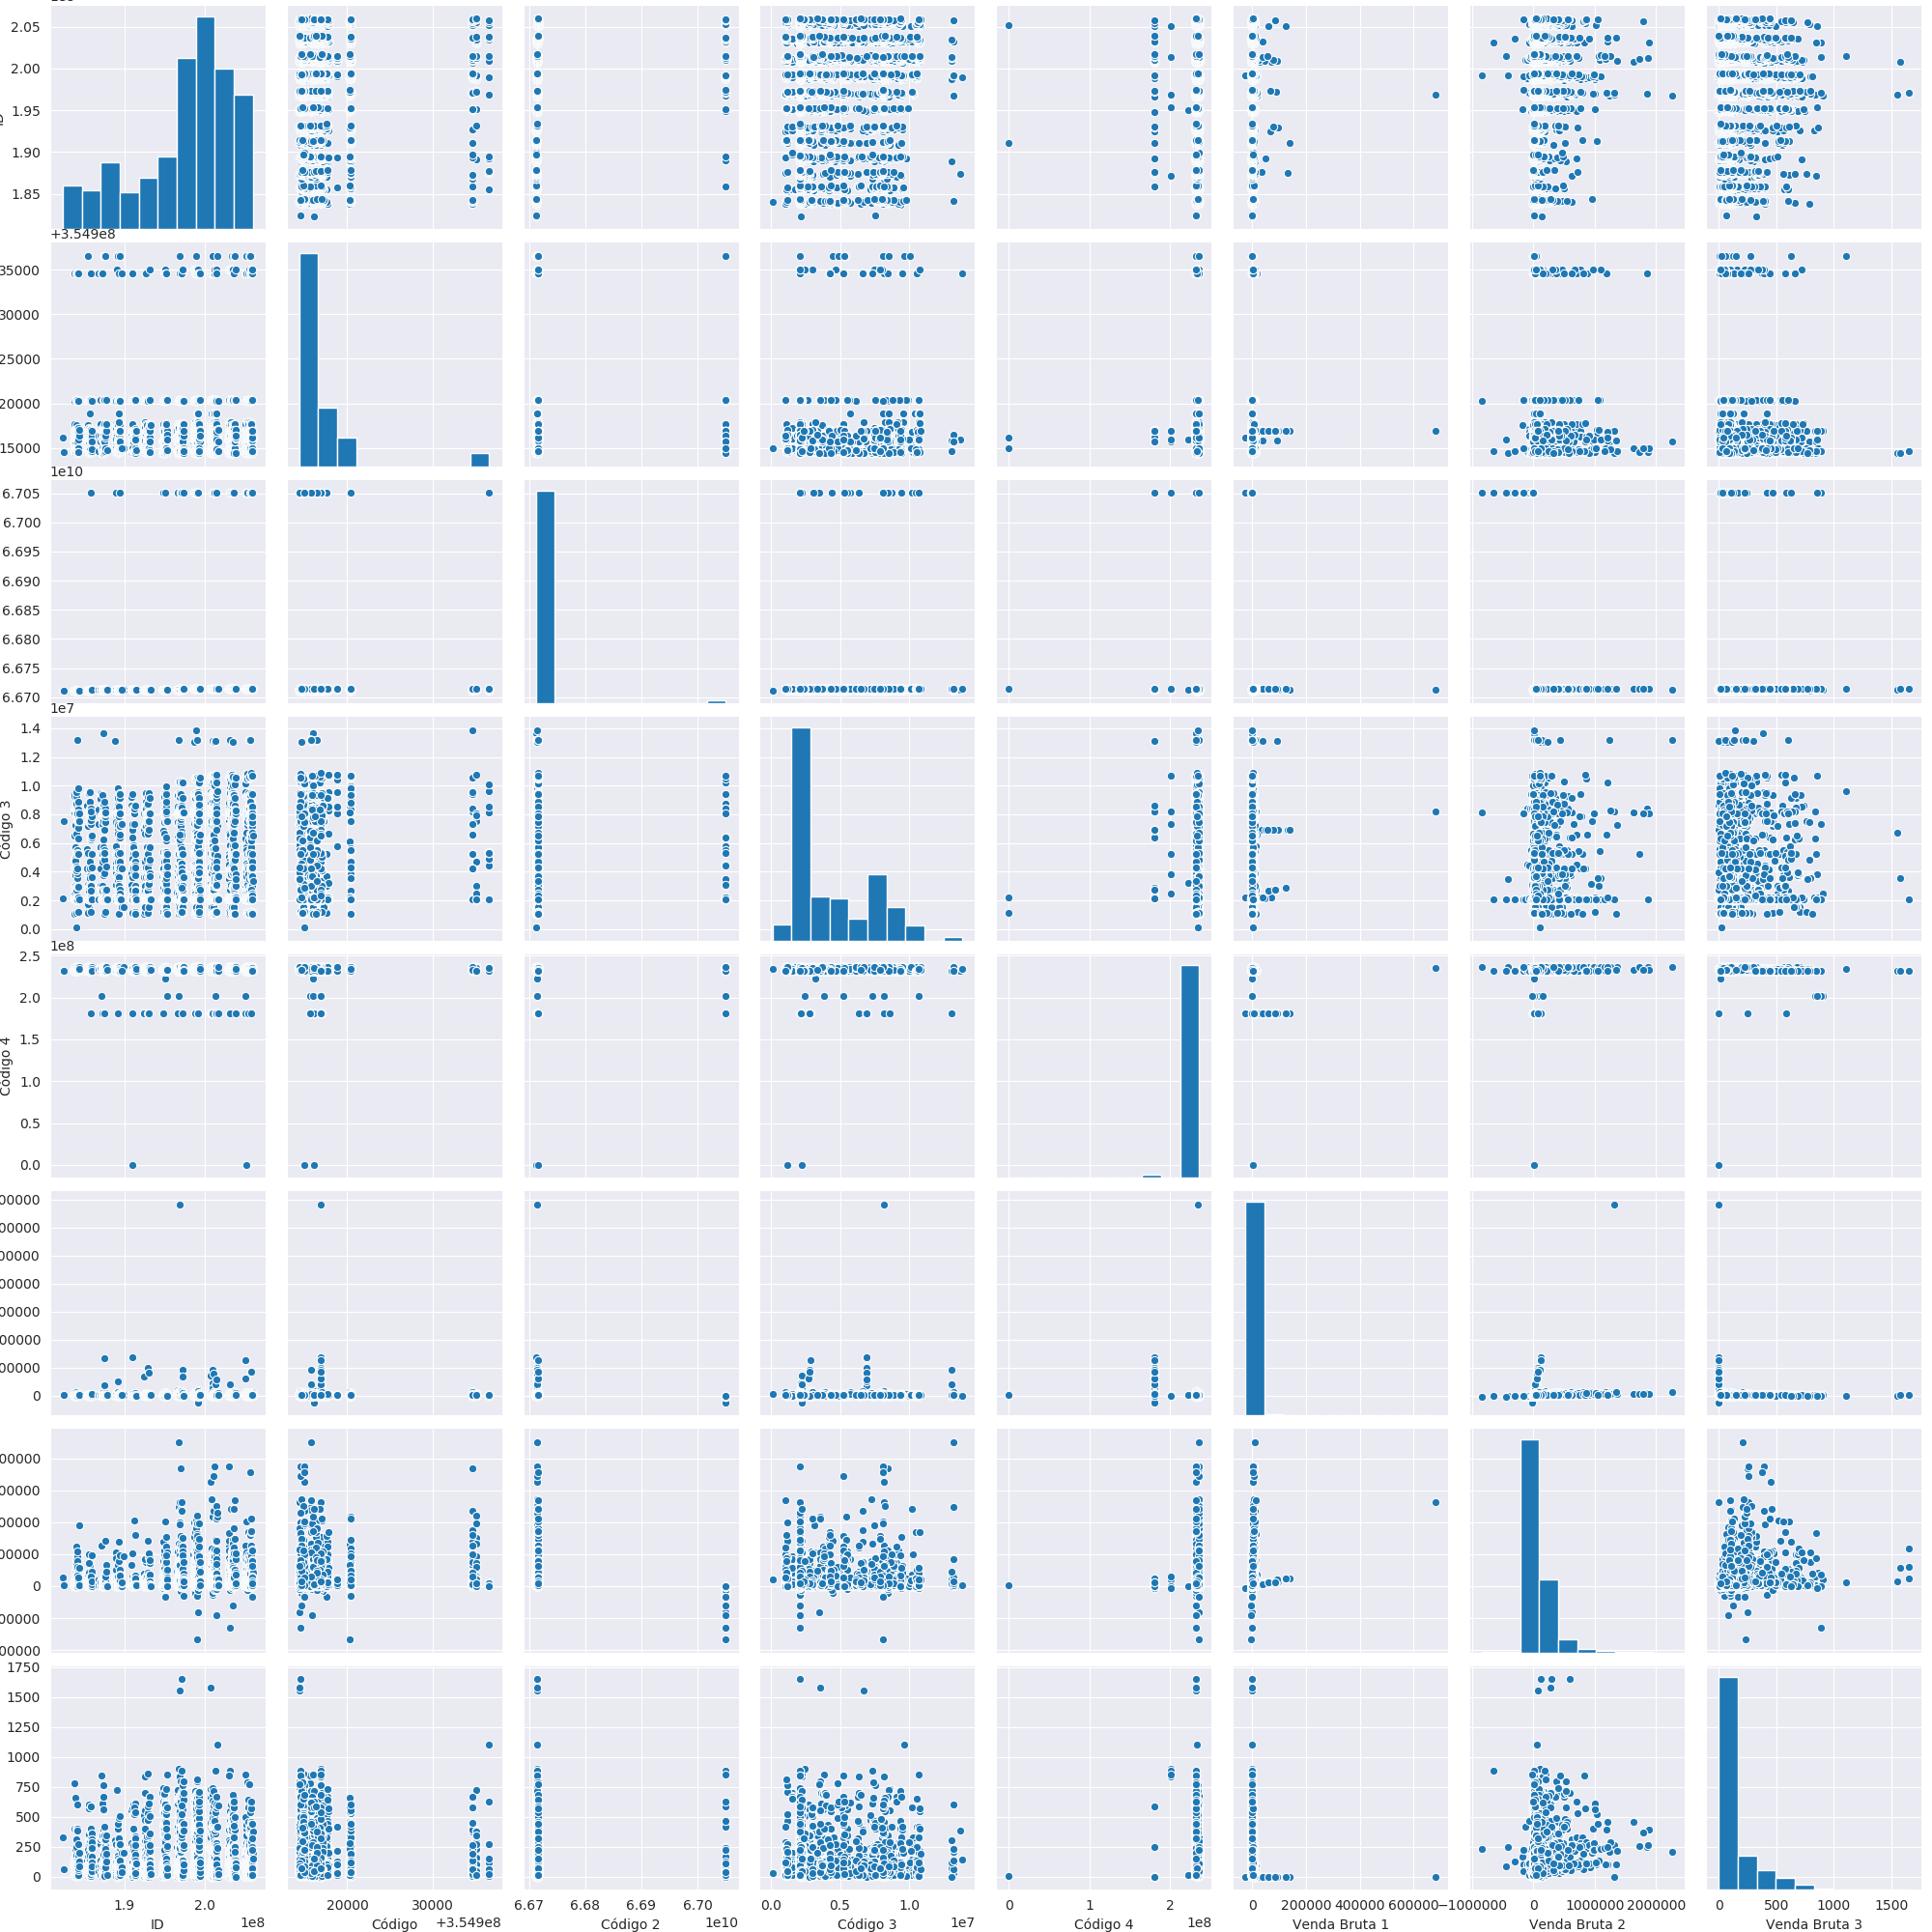
\includegraphics[scale=.16]{img/pair.png}
        \caption{Consequência da correlação fraca}
        \label{fig:pair1}
    \end{figure}
\end{frame}
\begin{frame}{}
    \begin{itemize}
        \item Remover dados irrelevantes para o aprendizado, como o ID;
        \item Preparação para realizar a Codificação de Categorias (Categorical Encoding):
        \begin{itemize}
            \item Alguns algoritmos do Python não conseguem ler dados categóricas;
            \item Associar dados categóricos a dados;
            \item Disponível apenas na v2 do programa.
            \item Ambas versões estão no GitHub.
        \end{itemize}
        \item Box plot para verificar outliers;
        \item Os mesmos passos são tomados no segundo versionamento do programa;
    \end{itemize}
\end{frame}

\begin{minted}{python}

df3 = df.drop(['ID', 'D#', 'Código',
    'Código 2', 'Código 3','Código 4'],axis=1)

#Remover outliers em atributos categóricos
#(os que só aparecem uma vez ou são desconhecidos)

df3=df3[df3['Produto 1'].apply(lambda x:
    x!= df3['Produto 1'].max())]
    
df3 = df3[df3['Tipo de venda'].apply(lambda x:
    x!='[Gr.Cliente Não Encontrado]')]

df3 = df3[df3['Produto 2'].apply(lambda x:
    False if x=='[Cultura Não Encontrada]'
    else (False if x=='[Cultura Não Especificada]'
    else True))]

df3 = df3[df3['Produto 1'].apply(lambda x:
    x!='[Gr Segmento Não Encontrado]')]

\end{minted}

\begin{frame}{}
    \begin{figure}
        \centering
        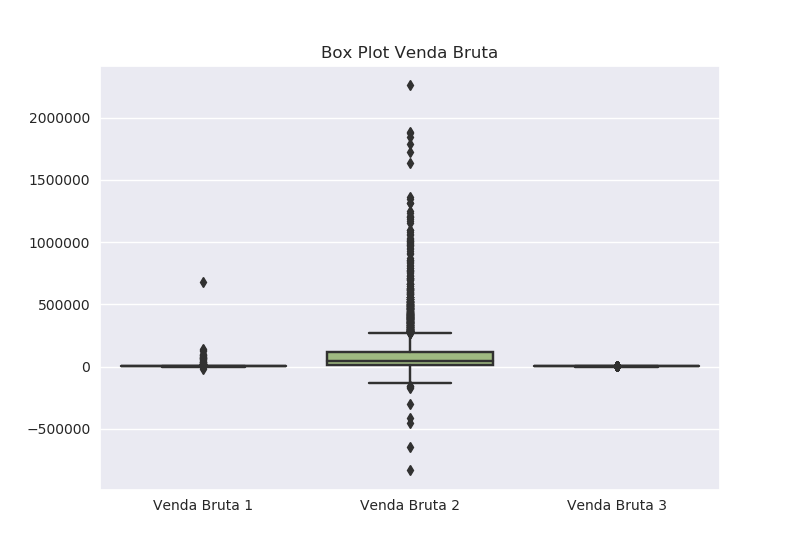
\includegraphics[scale=.5]{img/Box plot venda.png}
    \end{figure}
\end{frame}

\begin{minted}{python}
#
#
#

df3 = df3[df3['Venda Bruta 1'] !=
    df3['Venda Bruta 1'].max()]
    
df3 = df3[df3['Venda Bruta 2'] !=
    df3['Venda Bruta 2'].max()]
    
df3 = df3[df3['Venda Bruta 2'] !=
    df3['Venda Bruta 2'].min()]
    
df3 = df3[df3['Venda Bruta 2']  !=
    df3['Venda Bruta 2'].min()]
    
#recriar coluna de mês e outra do dia, o ano não
#todas as instâncias ocorrem no mesmo ano.

df3['Mês'] = df3['Data/Hora Dia'].apply(lambda x:
    x.month)

df3['Dia'] = df3['Data/Hora Dia'].apply(lambda x:
    x.day)

#remover atributo do tipo datetime
#algoritmo não lê.

#remover data hora dia
df3.drop('Data/Hora Dia',axis=1,inplace=True)    

\end{minted}


\begin{frame}{}
    \begin{itemize}
        \item Problema na coluna ABC, alguma das entradas não é um str, devemos remover essa entrada para realizar o label encoder;
        \item Classe d3info criada para verificar a variedade dos atributos e possivelmente aplicar one hot encoder.
    \end{itemize}
\end{frame}

\begin{minted}{python}
df3 = df3[df3['ABC'].apply(lambda x:
    False if type(x)!= np.str else True)]
    
df3info.tipo_venda
df3info.Produto_1
df3info.Produto_2

#tipo_venda possui 4 categorias, os outros mais de 4.
\end{minted}

\begin{frame}{}
    \begin{itemize}
        \item Esse modelo consistirá num diagnóstico de oportunidade de vendas, ele visa otimizar as transações realizadas.
        \item Dados indicam que a venda bruta total é bem alta;
        \item Quais condições provocam uma venda bem sucedida (acima da média);
        \item Suposição:
        \begin{align*}
            L=\sum_{i=1}^{3}{Vl}_i
        \end{align*}
            \begin{itemize}
                \item A classe será o lucro que consiste na soma dos três últimos atributos, que por hipótese, são o lucro líquido produzido pela compra.
            \end{itemize}
    \item Separar dados previsores dos dados classificadores;
    \item Realizar o label encoder;
    \end{itemize}
    
\end{frame}
\begin{minted}{python}
#
#

df3['Lucro'] = df3['Venda Bruta 1']+df3['Venda Bruta 2']
    +df3['Venda Bruta 3']

#classe LabelEncoder do sklearn

labelencoder = LabelEncoder()


#dados previsores:
previsores2 = df3.drop(['Venda Bruta 1',
        'Venda Bruta 2', 'Venda Bruta 3',
        'Lucro'], axis=1).values





#Label Encoder aos dados categóricos
for n in [1,2,4,3,5]:
  previsores2[:,n] =
  labelencoder.fit_transform(previsores2[:,n])
  
  
#One Hot Encoder em tipo de vendas

onehotencoder = make_column_transformer(
    (OneHotEncoder(categories='auto',
    sparse=False),[0]), remainder='passthrough')

X = onehotencoder.fit_transform(previsores2)

#Classe classificada como 0 caso x<mean e 1 x=> mean

classe2 = df3['Lucro'].apply(lambda x:
        0 if x < df3['Lucro'].mean() else 1)
\end{minted}

\begin{frame}{Treinamento dos modelos}
\begin{itemize}
    \item Dividir os dados em dados de treino e teste;
    \item Modelo treinado com 70\% dos dados e testado com 30\%;
    \item Treinar modelo de Naive Bayes Gaussiano e de Floresta Randômica;
    \item Verificar os dados testados e precisão do modelo;
\end{itemize}
\end{frame}

\begin{minted}{python}
#========================================
#   NAIVE BAYES GAUSSIANO
#========================================

#Carregar classe a partir do sklearn

nb2 = GaussianNB()

#Fitar o modelo
nb2.fit(X_treino2,Y_treino2)

#Testar o modelo
prev2 = nb2.predict(X_teste2)

#Taxas de acerto e erro

taxa_acerto2 = (accuracy_score(Y_teste2, prev2))*100
taxa_erro2 = (1 - taxa_acerto2/100)*100

#========================================
#   FLORESTA RANDOMICA
#========================================

#Carregar classe a partir do sklearn.ensemble

floresta2 = RandomForestClassifier(n_estimators =
    200)

#n_estimators é o número de árvores de decisão

#ajustar o modelo
floresta2.fit(X_treino2,Y_treino2)

#testar modelo
previsoes2 = floresta2.predict(X_teste2)


\end{minted}

\begin{frame}{Resultados}
\section{Resultados}
\begin{itemize}
    \item Verificar Taxas de acerto e de erro;
    \item Criar matriz de confusão do modelo;
    \begin{itemize}
        \item Métrica voltada para modelos de classificação;
        \item Quantidade de FP, FN, VP, VN;
        \item Acurácia e sensibilidade;
    \end{itemize}
\end{itemize}
\begin{figure}
    \centering
    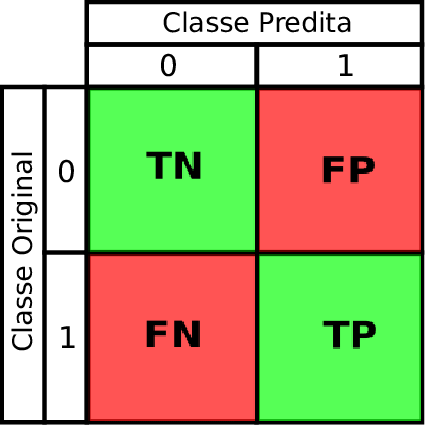
\includegraphics[scale=.2]{img/confusion.png}
    \caption{Tabela de Confusão}
    \label{fig:confusion}
\end{figure}
\end{frame}
\begin{frame}
    \begin{figure}
        \centering
        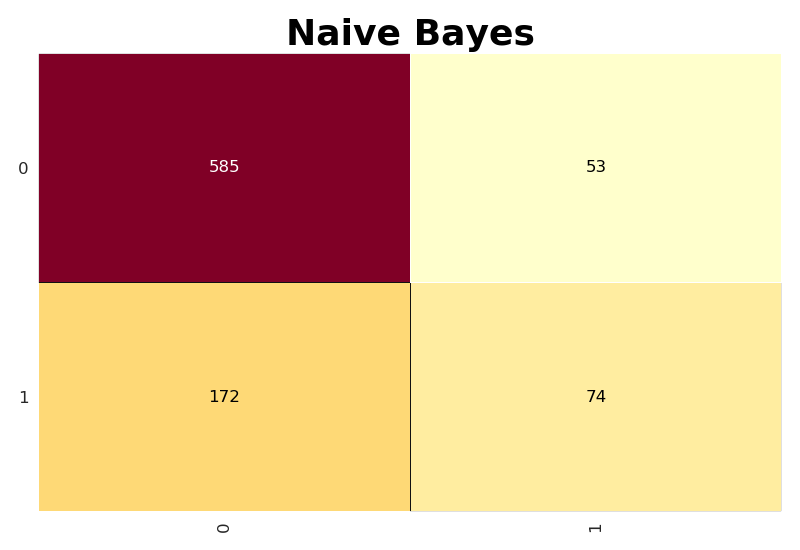
\includegraphics[scale=.5]{img/ConfusionMatrix Naive Bayes 2.png}
        \caption{Naive Bayes}
        \label{fig:my_label}
    \end{figure}
\end{frame}

\begin{frame}
    \begin{figure}
        \centering
        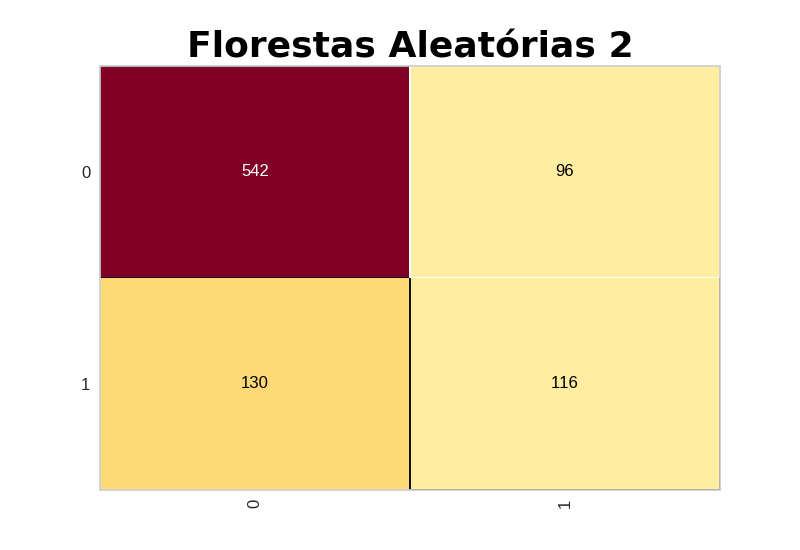
\includegraphics[scale=.5]{img/ConfusionMatrix Florestas.png}
        \caption{Naive Bayes}
        \label{fig:my_label}
    \end{figure}
\end{frame}

\section{Discussão}
\begin{frame}{Discussões}
    O modelo foi fitado com sucesso e apresentou as seguintes taxas:
    \begin{table}[h!]
        \centering
        \begin{tabular}{|c|c|c|}
            \hline
            Modelo &  Taxa de acerto & Taxa de erro\\
            \hline
            Naive Bayes & 74,55\%&  25,45\%\\
            \hline
            Ensemble & 74,77\% &25,23\%\\
            \hline
        \end{tabular}
    \end{table}
    
    As taxas da tabela acima implicam que o modelo foi bem treinado, mas levando em conta as hipóteses que foram tomadas. Obtendo acesso à mais informações sobre a lista, pode ser necessário recorrer a outros modelos de aprendizado.
\end{frame}
\section{Otimização}
\begin{frame}{Otimização}
    O modelo pode ser otimizado levando em conta os valores reais dos atributos que não foram informados e tomando considerações reais sobre os valores do lucro bruto que não pode ser contabilizada devido à falta de informação
\end{frame}





%%% BIBLIOGRAFIA %%%
\begin{frame}[allowframebreaks]
\frametitle{Referências}
\bibliographystyle{plain}
\bibliography{referencias.bib}
\end{frame}



\end{document}
